\begin{frame}
  \centering
  \textbf{\Large{Chemistry with Multiwavelets}}
\end{frame}

\begin{frame}
  \frametitle{One-electron systems}
  \centering
  \textbf{Schr\"{o}dinger equation}
  \begin{equation}
    %\nonumber
    \bigg[-\frac{1}{2}\nabla^2 + \potential\bigg]\wavefunction(r) = E \wavefunction(r)
  \end{equation}

  \vspace{5mm}

  \textbf{Rewrite using} $\mu^2 = -2E$
  \begin{align}
    %\nonumber
    \Big[-\nabla^2 + \mu^2\Big]\wavefunction(r) =&\ -2 \potential \wavefunction(r)\\
    %\nonumber
    \wavefunction(r) =&-2\Big[-\nabla^2 + \mu^2\Big]^{-1} \potential \wavefunction(r)\\
    %\nonumber
    \wavefunction =&-2\Helm\Big[\potential \wavefunction\Big]
  \end{align}

  \vspace{5mm}

  \textbf{Bound-State Helmholtz operator}
  \begin{equation}
    %\nonumber
    \Helm f(r) = \Big[-\nabla^2 + \mu^2\Big]^{-1} f(r) = \int \frac{e^{-\mu |r-r'|}}{4\pi|r-r'|}f(r')dr'
  \end{equation}

  \vspace{5mm}

  \centering
  \tiny
  MH Kalos,
  {\it Phys. Rev.},
  \textbf{128(4)},
  1791 (1962)\\
  RJ Harrison, GI Fann, T Yanai, Z Gan and G Beylkin,
  {\it J. Chem. Phys.},
  \textbf{121},
  11587 (2004)
\end{frame}

\begin{frame}
  \frametitle{One-electron systems}
  \centering
  \textbf{Power iteration of the BSH operator}
  \begin{equation}
    %\nonumber
    \wavefunction^{n+1} = -2\Helm^n\Big[\potential \wavefunction^n\Big]
  \end{equation}

  \vspace{3mm}

  \textbf{Finding roots of the residual}
  \begin{equation}
    %\nonumber
    f(\wavefunction) = -2\Helm^n\big[\potential \wavefunction\big] - \wavefunction
  \end{equation}

  \vspace{3mm}

  \textbf{Newton's method}
  \begin{align}
    \wavefunction^{n+1} &= \wavefunction^n - \Big[J(\wavefunction^n)\Big]^{-1} f(\wavefunction^n)\\
    \wavefunction^{n+1} &= \wavefunction^n - \Big[J(\wavefunction^n)\Big]^{-1}
    \bigg(-2\Helm^n\Big[\potential \wavefunction^n\Big] - \wavefunction^n\bigg)
  \end{align}

  \vspace{3mm}

  \begin{itemize}
    \item Direct power iteration is an "inexact" Newton method with Jacobian $J(\wavefunction^n) \approx -1$.
    \item Krylov Accelerated Inexact Newton (KAIN) method accelerates convergence
    \item Similar in spirit to Direct Inversion of Iterative Subspace (DIIS)
  \end{itemize}
\end{frame}

\begin{frame}
  \frametitle{Example: Hydrogen atom}
  \begin{columns}
    \begin{column}[b]{0.4\textwidth}
      \centering
      \textbf{Construct BSH $\Helm$ using}
      \begin{equation}
        \nonumber
        \mu = \sqrt{-2E_H}, \qquad  E_H = -\frac{1}{2}
      \end{equation}

      \vspace{2mm}

      \textbf{Power iteration}
      \begin{equation}
        \nonumber
        \tilde{\wavefunction}^{n+1} = -2\Helm \Big[\potential \wavefunction^n \Big]
      \end{equation}

      \vspace{2mm}

      \textbf{Compute residual}
      \begin{equation}
        \nonumber
        \Delta\tilde{\wavefunction}^{n} = \tilde{\wavefunction}^{n+1} - \wavefunction^n
      \end{equation}

      \vspace{2mm}

      \textbf{Normalize}
      \begin{equation}
        \nonumber
        \wavefunction^{n+1} = \frac{\tilde{\wavefunction}^{n+1}}{||\tilde{\wavefunction}^{n+1}||^2}
      \end{equation}

      \vspace{3mm}

    \end{column}
    \begin{column}[b]{0.6\textwidth}
      \centering
      \textbf{Potential operator}
      \begin{equation}
        \nonumber
        \potential = \nuclear(r) = -\frac{1}{|r-R|}
      \end{equation}
      \begin{center}
        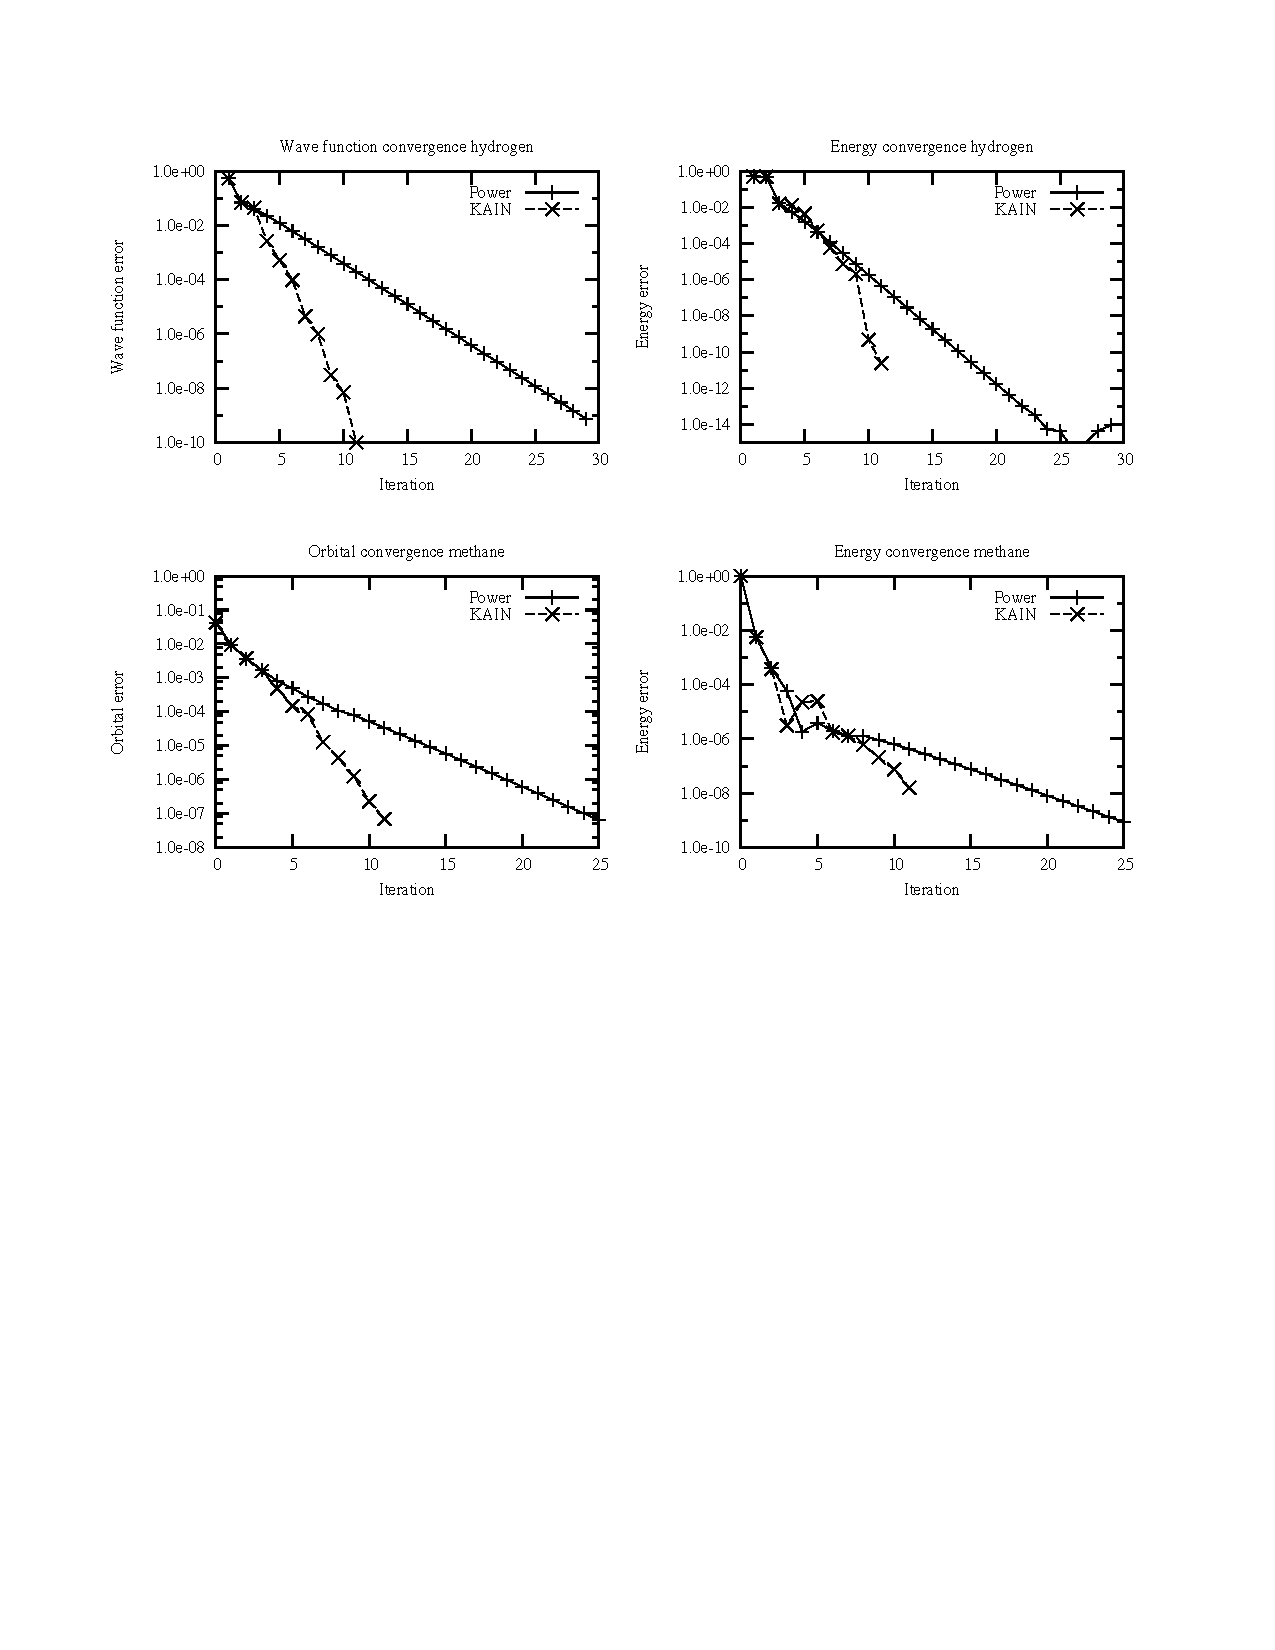
\includegraphics[scale=0.8, clip, viewport = 50 550 300 730]{figures/convergence.pdf}
      \end{center}
    \end{column}
  \end{columns}
\end{frame}

\begin{frame}
  \frametitle{Example: Hydrogen atom}

  \textbf{LCAO:}
  \begin{itemize}
    \item Algebraic problem that is an \emph{approximation} (projection) of the physical model
    \item Finding "exact" solution to \emph{approximate} problem (constraints of fixed basis)
    \item Virtual contributions rotated into occupied space
    \item Fixed potential $\rightarrow$ solution found in single iteration
    \item DIIS searches for optimal solution \emph{within} iterative subspace
  \end{itemize}

  \vspace{5mm}

  \textbf{MW:}
  \begin{itemize}
    \item Finding \emph{approximate} solution to \emph{exact} physical model
    \item Not a fixed basis, no virtual orbitals
    \item Need to "sample" virtual space by application of BSH Green's function
    \item Fixed potential \emph{still} requires iterative solution
    \item KAIN extrapolates solution \emph{outside} iterative subspace
  \end{itemize}
\end{frame}

\begin{frame}
    \frametitle{Energy calculation}
    \begin{itemize}
        \item Power iteration converges the $(\psi, E)^n$ \emph{pair}
        \vspace{4mm}
        \item Need to update the energy ($\mu^n = \sqrt{-2E^n}$) to achieve convergence:
        \vspace{4mm}
        \begin{enumerate}
            \item Straightforward way:
                $E^n = -\frac{1}{2} \langle \psi^n|\nabla^2 \psi^n \rangle + \langle \psi^n|\potential \psi^n \rangle$
            \vspace{2mm}
            \item Symmetric kinetic:
                $E^n = \frac{1}{2} \langle \nabla \psi^n|\nabla \psi^n \rangle + \langle \psi^n|\potential \psi^n \rangle$
            \vspace{2mm}
            \item Direct update w/o kinetic operator:
                $E^n = E^{n-1} + F(\potential, \psi^n, \psi^{n-1})$
        \end{enumerate}
        \vspace{4mm}
        \item Remember, we don't like derivatives!
        \vspace{4mm}
        \item Exercise: Derive energy expression $F$ in (3)
    \end{itemize}
\end{frame}

\begin{frame}
  \frametitle{Many-electron systems}
  \begin{itemize}
    \item Kohn-Sham/Hartree-Fock equations:
      \begin{equation}
        \left[-\frac{1}{2}\nabla^2 + \potential\right] \orbital_i(r) = \epsilon_i \orbital_i(r)
      \end{equation}
    \item Iterate integral form for each orbital separately:
      \begin{equation}
       \tilde{\orbital}_i^{n+1} = -2\Helm_i^n\left[\potential^n \orbital_i^n \right]
      \end{equation}
    \item With potential operator that depend on the orbitals:
      \begin{equation}
        \potential^n = \nuclear + \coulomb^n + \xc^n - \lambda\exchange^n, \qquad 0 \leq \lambda \leq 1
      \end{equation}
    \item Straightforward iteration will converge \emph{all} orbitals to the lowest energy eigenfunction
    \vspace{4mm}
    \item Need to \emph{orthogonalize} the orbitals to fill the $N$ \emph{lowest} energy eigenfunctions
      \begin{equation}
        \orbital_i = \Big(1 - \sum_{j<i}|\orbital_j\rangle\langle\orbital_j|\Big)\tilde{\orbital}_i
        %\orbital_i = \sum_j \tilde{S}_{ij}^{-1/2} \tilde{\orbital}_j, \qquad \tilde{S}_{ij} = \langle \tilde{\orbital}_i | \tilde{\orbital}_j \rangle
      \end{equation}
  \end{itemize}
\end{frame}

\begin{frame}
  \frametitle{Many-electron systems}
  \centering
  \normalsize
  \textbf{Potential operator} $0 \leq \lambda \leq 1$
  \begin{equation}
    \nonumber
    \potential = \nuclear + \coulomb + \xc - \lambda\exchange
  \end{equation}

  \vspace{8mm}

  \begin{columns}
    \begin{column}[b]{0.5\textwidth}
      \centering
      \textbf{Nuclear operator}
      \begin{equation}
        \nonumber
	    \nuclear \orbital_p(r) = \left(-\sum_I\frac{Z_I}{|r-R_I|}\right) \orbital_p(r)
      \end{equation}
    \end{column}

    \begin{column}[b]{0.5\textwidth}
      \centering
      \textbf{Exchange-Correlation operator}
      \begin{equation}
        \nonumber
        \xc \orbital_p(r) = \left(\frac{\delta E_{xc}}{\delta \rho}\right) \orbital_p(r)
                  %= \frac{\partial F_{xc}}{\partial \density} 
                  %- \nabla \cdot \frac{\partial F_{xc}}{\partial \nabla\density}
      \end{equation}
    \end{column}
  \end{columns}

  \vspace{8mm}

  \centering
  \textbf{Coulomb operator}
  \begin{equation}
    \nonumber
    %\elPot(r) = \int \frac{\density(r')}{|r-r'|} \ud r'
    \coulomb\orbital_p(r) = \sum_i \orbital_p(r) \int \frac{\orbital_i^\dagger(r')\orbital_i(r')}{|r-r'|} \ud r'
                          %= \sum_i \orbital_i(r) \Poisson{4\pi\orbital_i^\dagger \orbital_p}
                          = \Poisson{4\pi\density} \orbital_p(r)
  \end{equation}

  \vspace{5mm}

  \centering
  \textbf{Exchange operator}
  \begin{equation}
    \nonumber
    \exchange\orbital_p(r) = \sum_i \orbital_i(r) \int \frac{\orbital_i^\dagger(r')\orbital_p(r')}{|r-r'|} \ud r'
                           = \sum_i \orbital_i(r) \Poisson{4\pi\orbital_i^\dagger \orbital_p}
  \end{equation}
\end{frame}

\begin{frame}
  \frametitle{Example: Small atoms}
  \begin{columns}
    \begin{column}[b]{0.4\textwidth}
      \small
      \centering
      \textbf{Construct potential operator}
      \begin{equation}
        \nonumber
        \potential^n = \nuclear^n + \coulomb^n + \xc^n + \lambda\exchange^n
      \end{equation}

      \vspace{2mm}

      \textbf{Compute Fock matrix}
      \begin{equation}
        \nonumber
        F_{ij}^{n} = \langle\orbital_i^{n}|\kinetic + \potential^n|\orbital_j^{n}\rangle
      \end{equation}

      \vspace{2mm}

      \textbf{Diagonalize Fock matrix}
      \begin{equation}
        \nonumber
        F_{ij}^n \rightarrow \epsilon_i^n
      \end{equation}

      \vspace{2mm}

      \textbf{Construct BSH $\Helm_i^n$ using}
      \begin{equation}
        \nonumber
        \mu_i^n = \sqrt{-2\epsilon_i^n}
      \end{equation}

      \vspace{2mm}

      \textbf{Power iteration}
      \begin{equation}
        \nonumber
        \tilde{\orbital}_i^{n+1} = -2\Helm_i^n \left[\potential^n \orbital_i^n\right]
      \end{equation}

      \vspace{2mm}

      \textbf{Orthonormalize}
      \begin{equation}
        \nonumber
        \orbital_i^{n+1} = \Big(1 - \sum_{j<i}|\orbital_j^{n+1}\rangle\langle\orbital_j^{n+1}|\Big)\tilde{\orbital}_i^{n+1}
      \end{equation}

      \vspace{2mm}

    \end{column}
    \begin{column}[b]{0.6\textwidth}
      \centering
      \small
      \textbf{Overall accuracy kept at} $\epsilon = 10^{-6}$
      \begin{center}
	    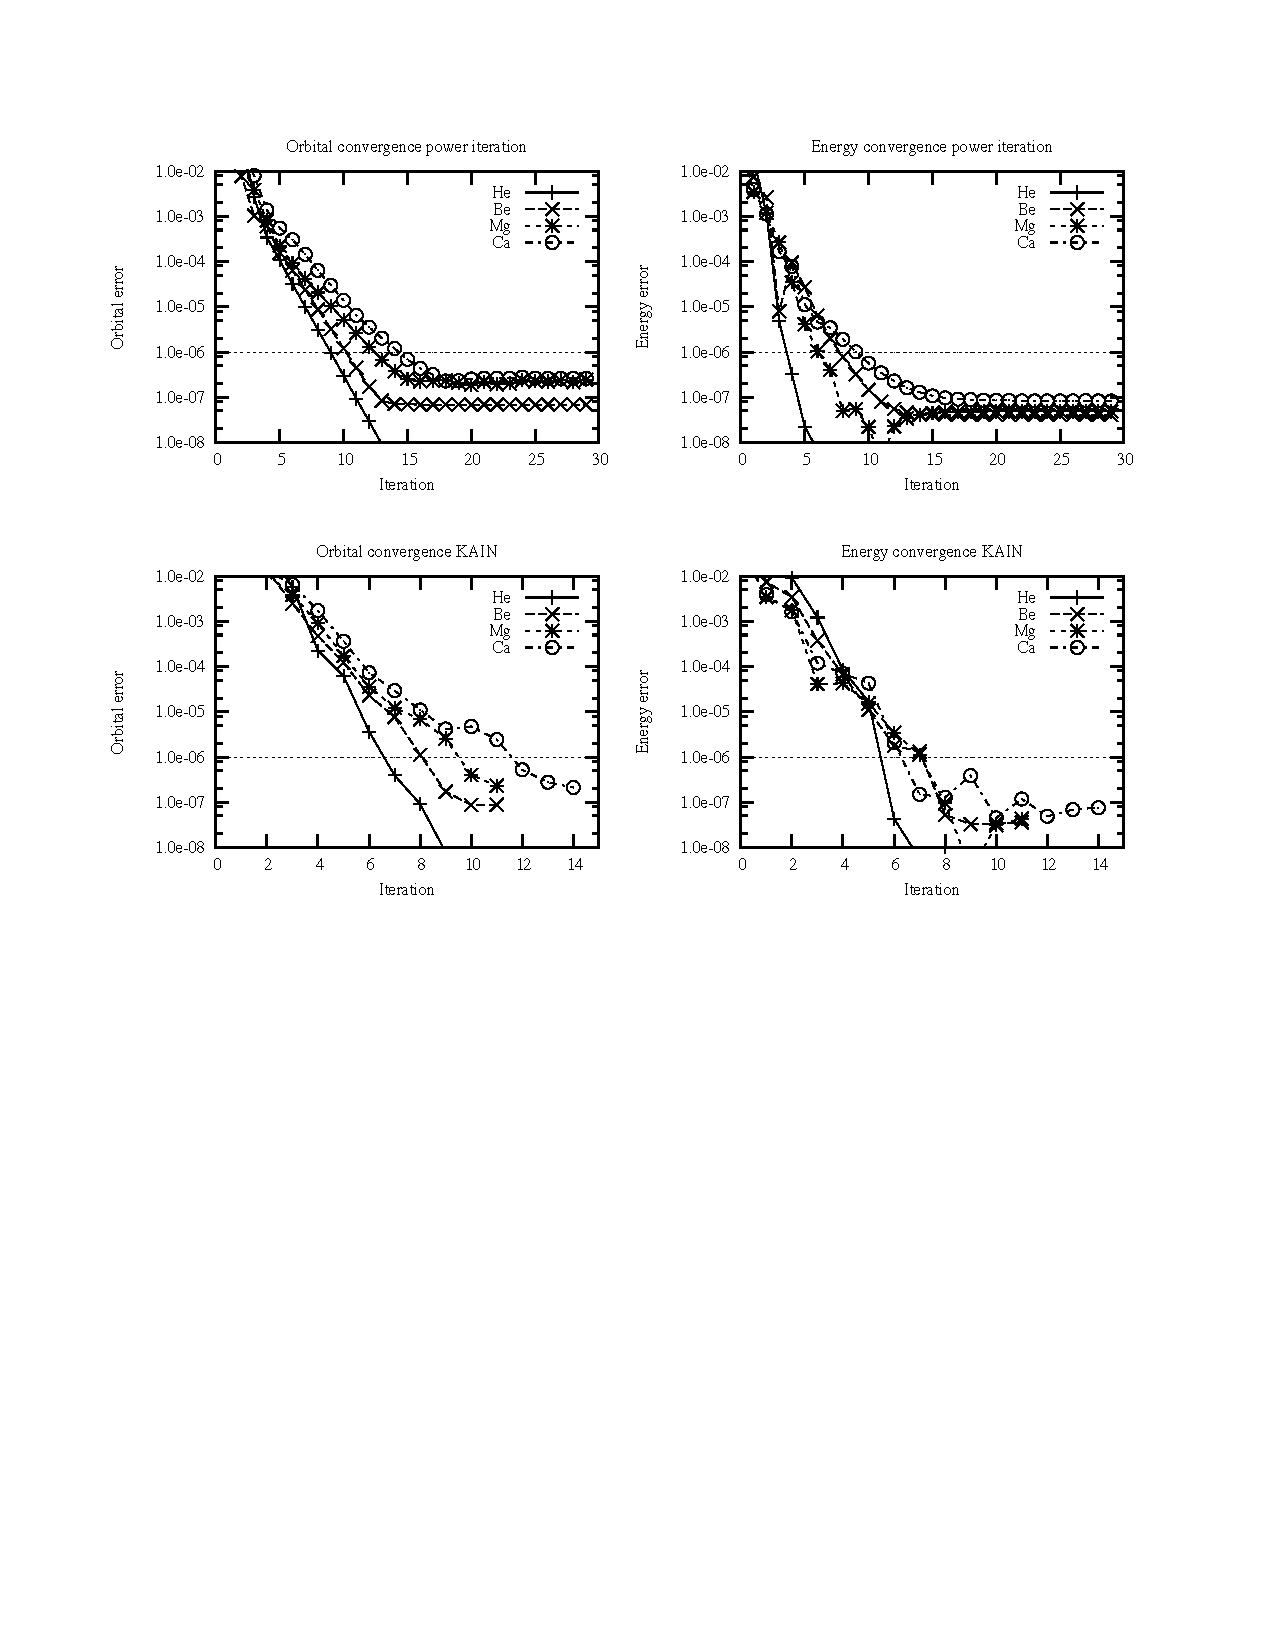
\includegraphics[scale=0.8, clip, viewport = 50 550 300 740]{figures/accuracy.pdf}
      \end{center}
      \vspace{10mm}
    \end{column}
  \end{columns}
\end{frame}

\begin{frame}
    \frametitle{Localized orbitals}
    \centering
    Total energy invariant under unitary transformations among occupied orbitals
    \begin{equation}
	\nonumber
	\phi_i = \sum_j L_{ij} \phi_i, \qquad \qquad L^\ast L = LL^\ast = I
    \end{equation}

    \begin{columns}
    \begin{column}[b]{0.48\linewidth}
    \centering
    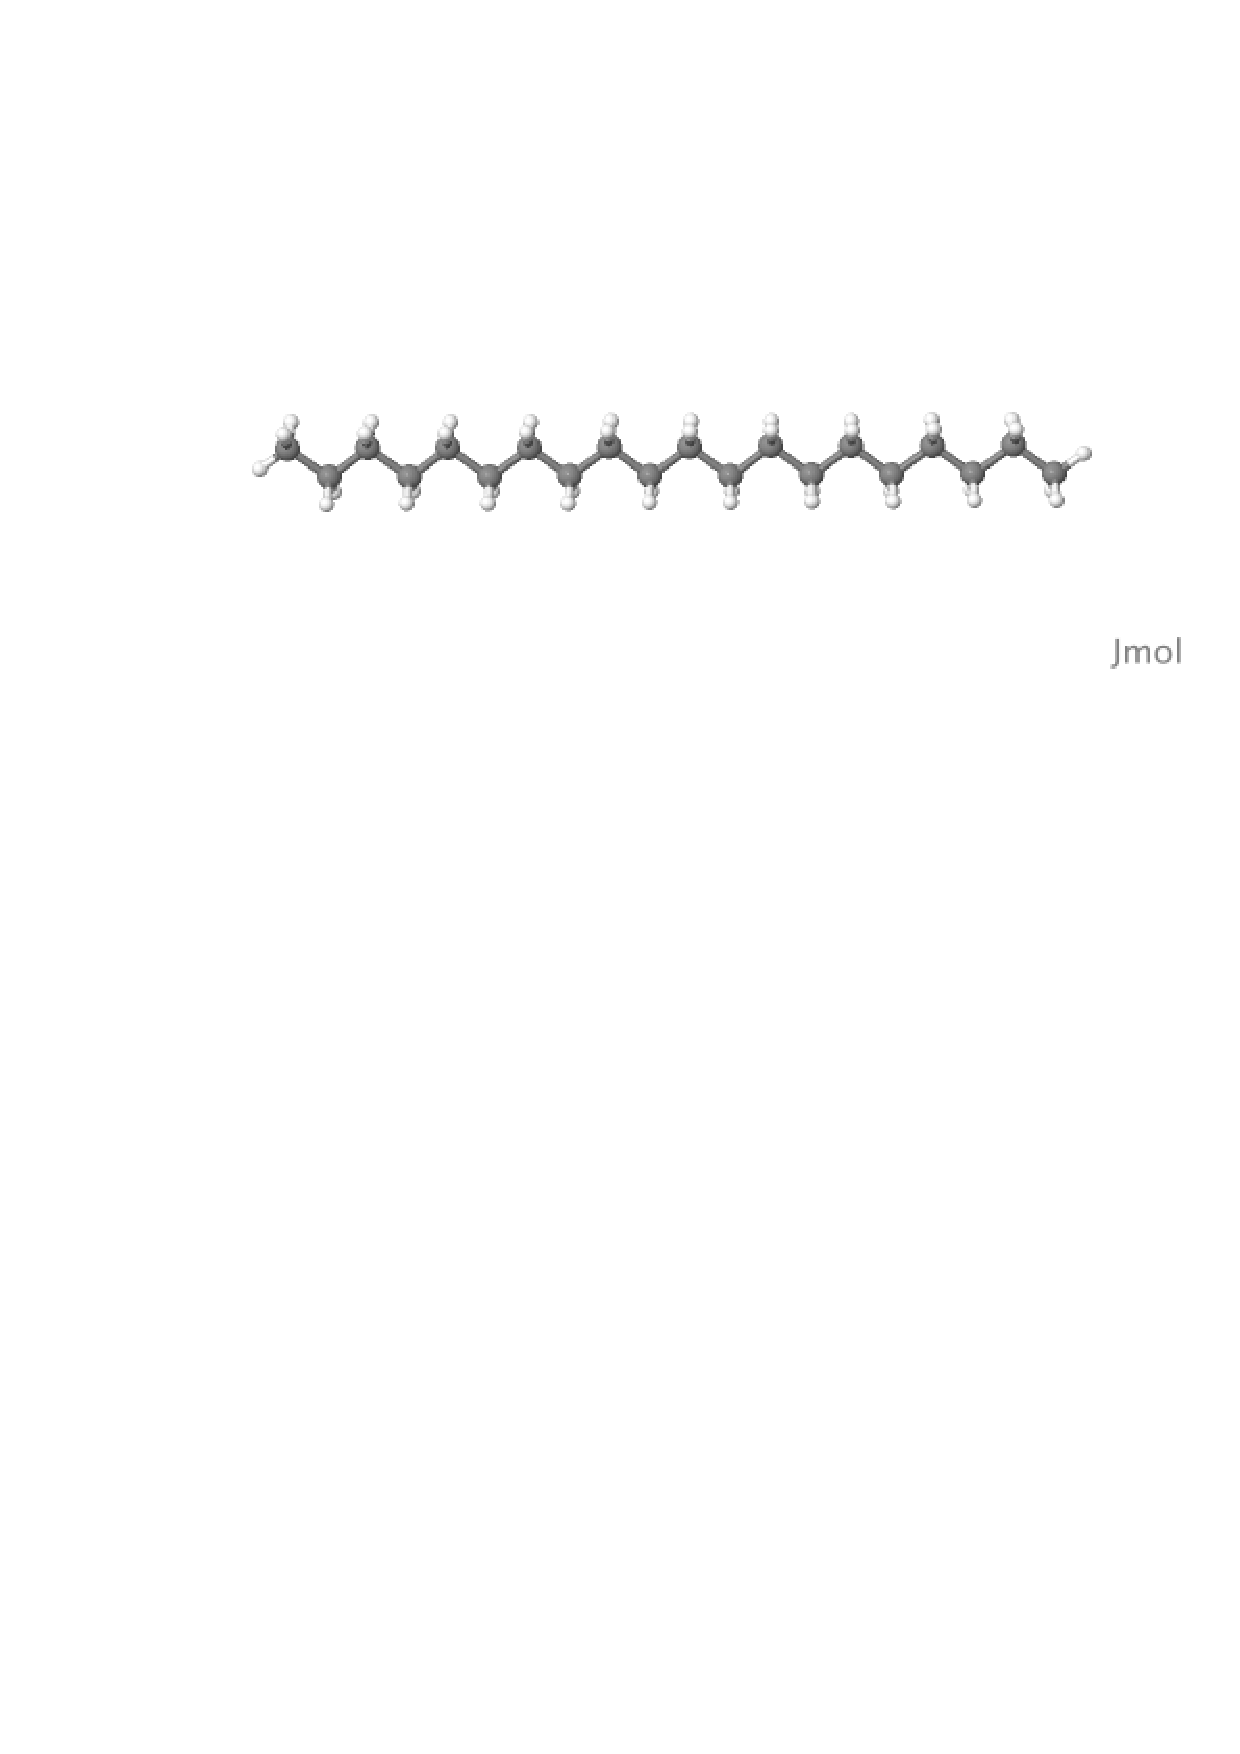
\includegraphics[scale=0.25, clip, viewport = 80 560 600 700]{figures/alkane.pdf}\\
    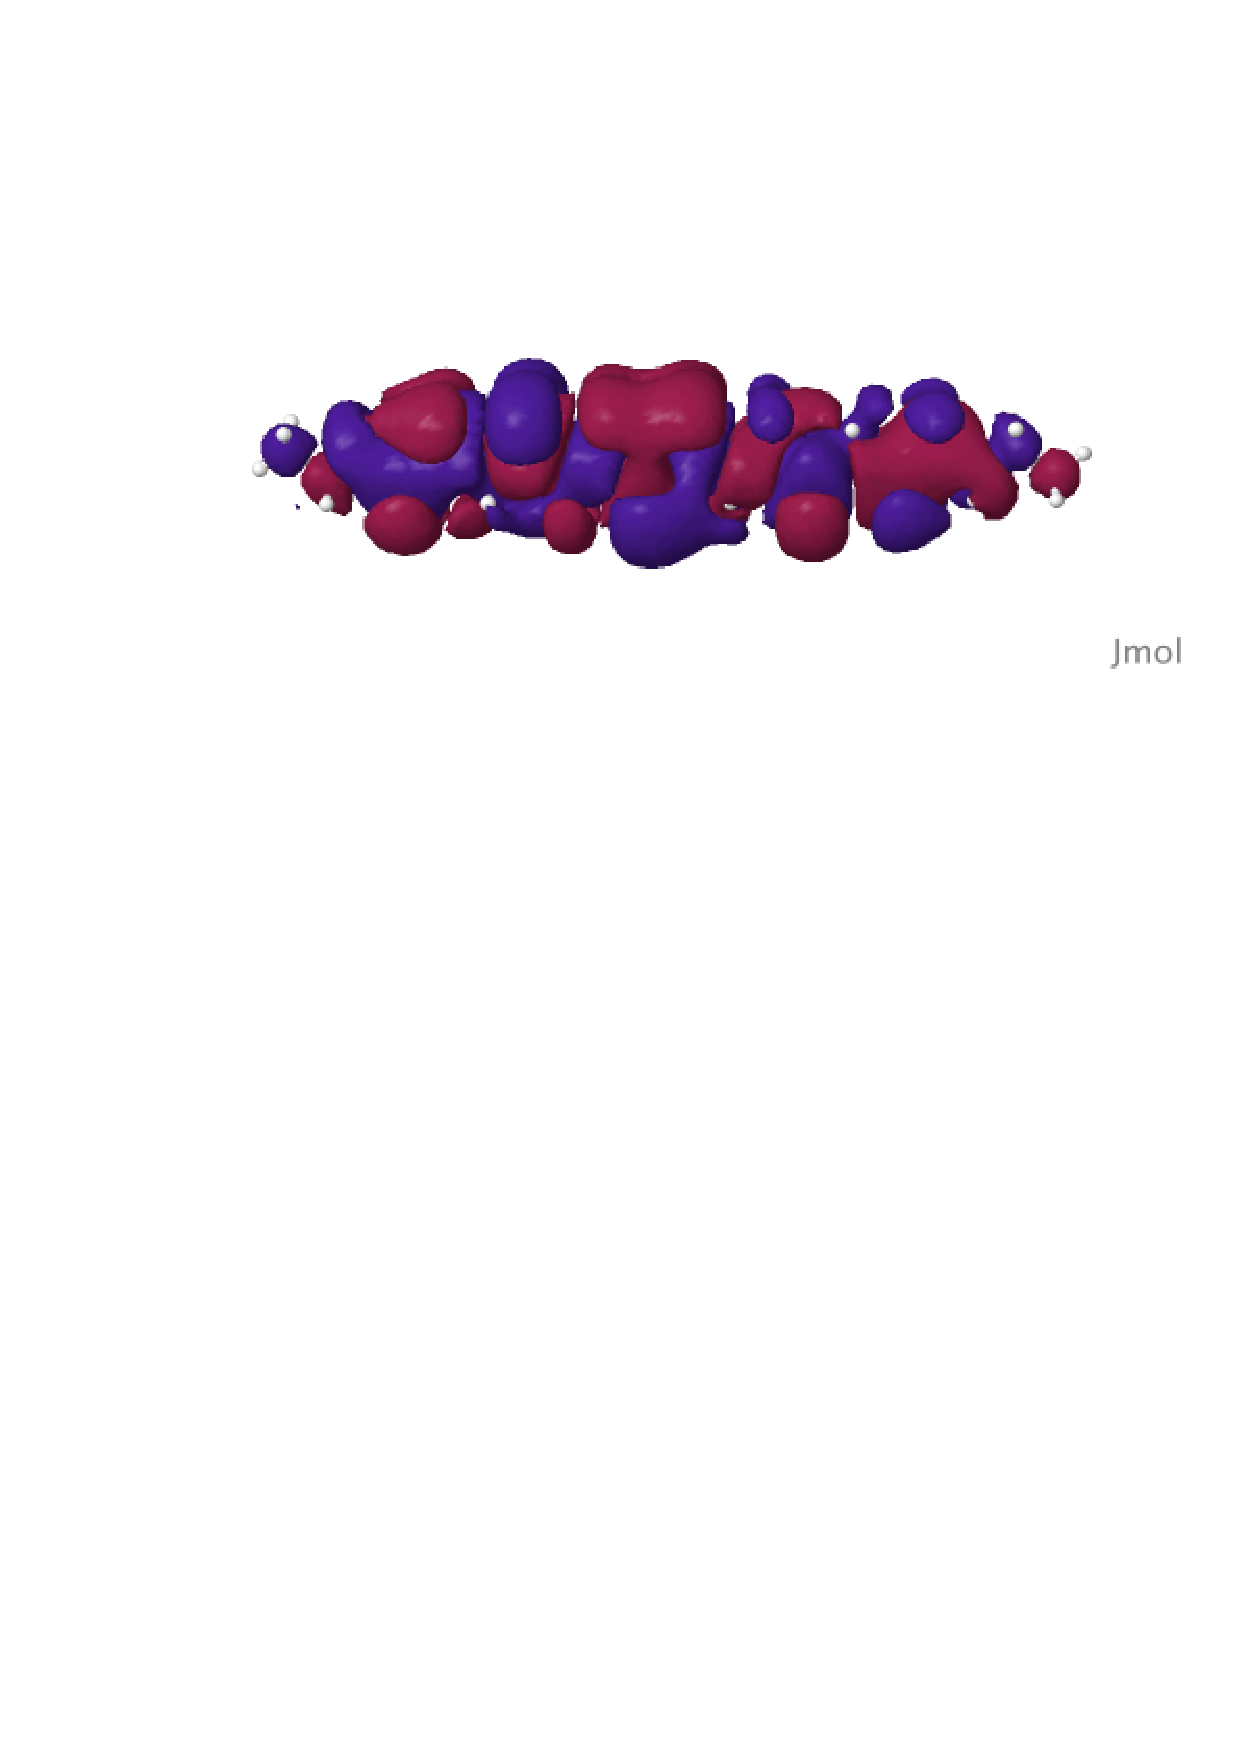
\includegraphics[scale=0.25, clip, viewport = 80 560 600 700]{figures/can_orb_1.pdf}\\
    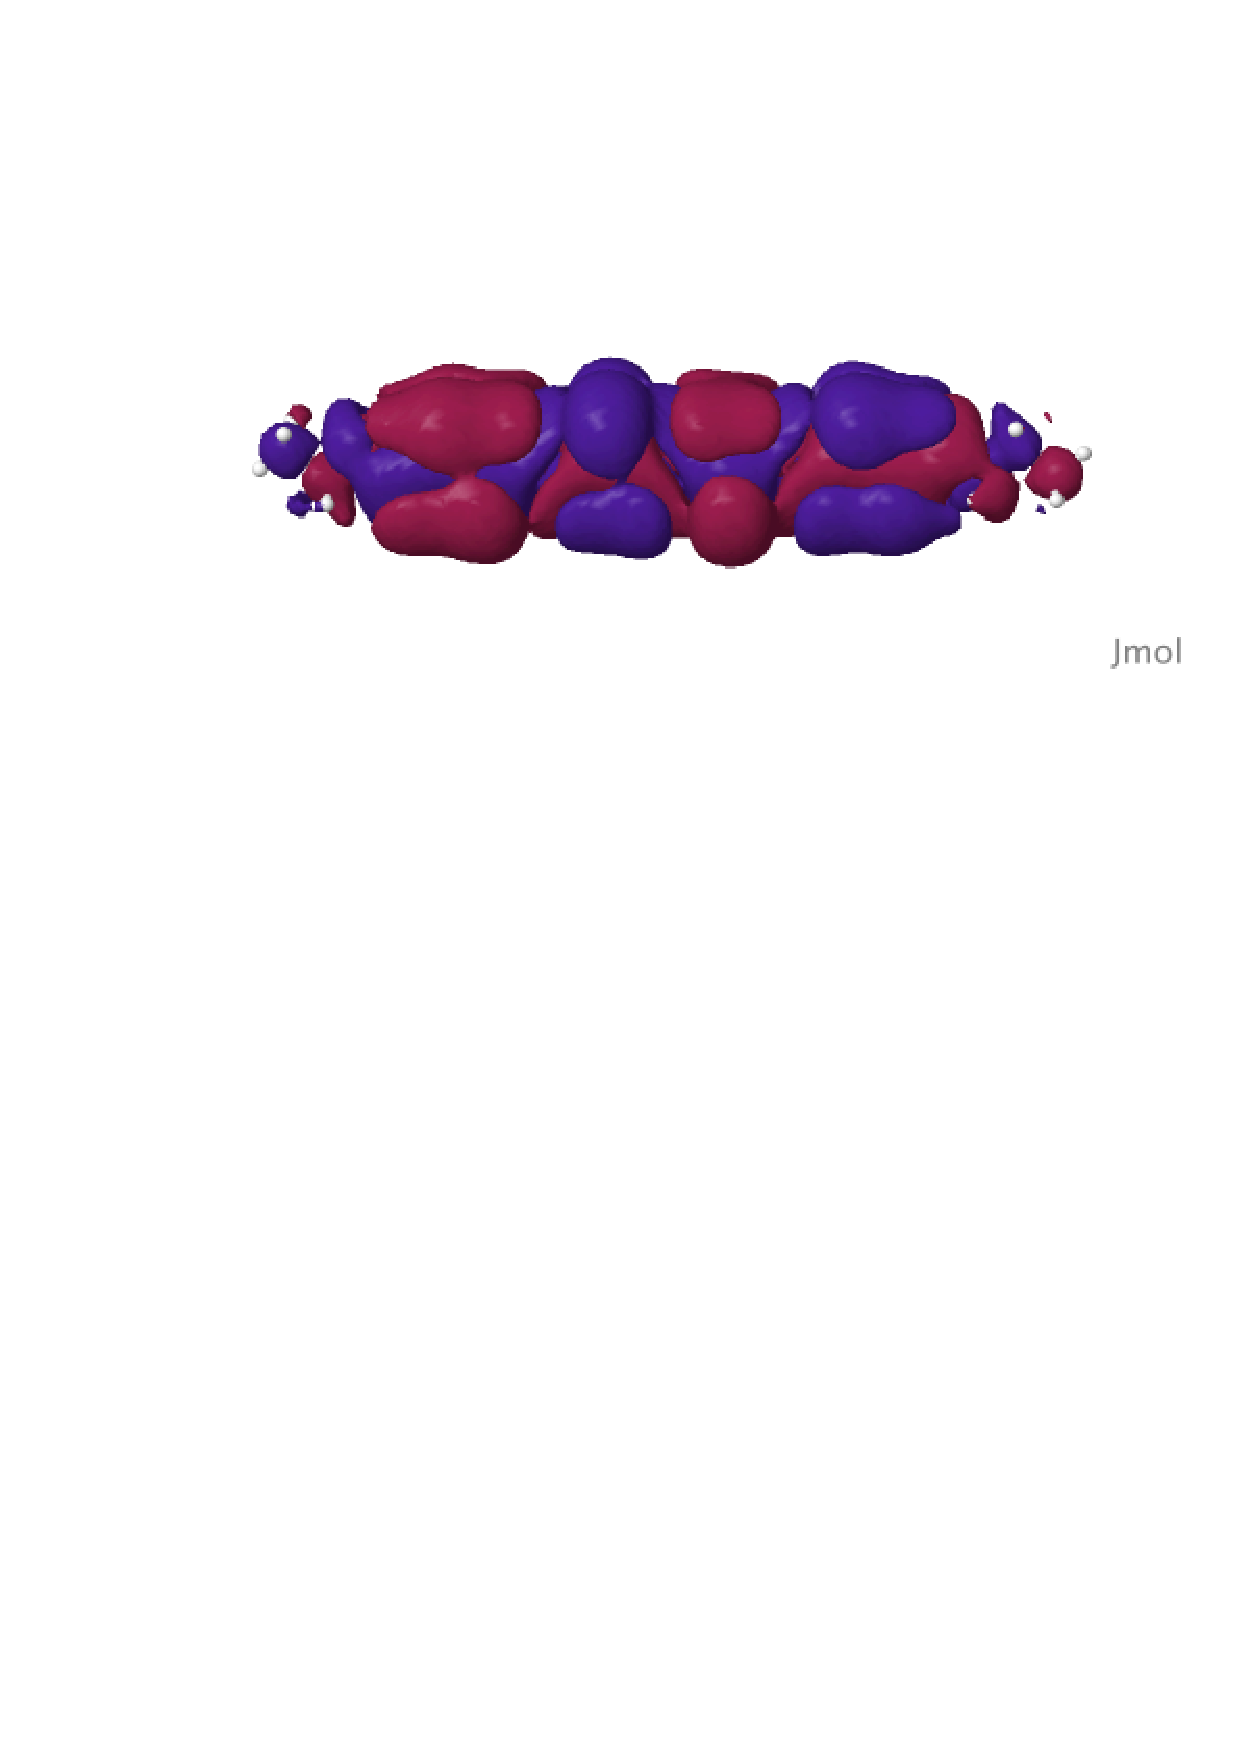
\includegraphics[scale=0.25, clip, viewport = 80 560 600 700]{figures/can_orb_2.pdf}\\

    \vspace{2mm}

    \begin{equation}
        \nonumber
        \orbital_i =\ -2\Helm_i\Bigg[\potential \orbital_i\Bigg]
    \end{equation}
    \end{column}

    \begin{column}[b]{0.48\linewidth}
\only<2>{
    \centering
    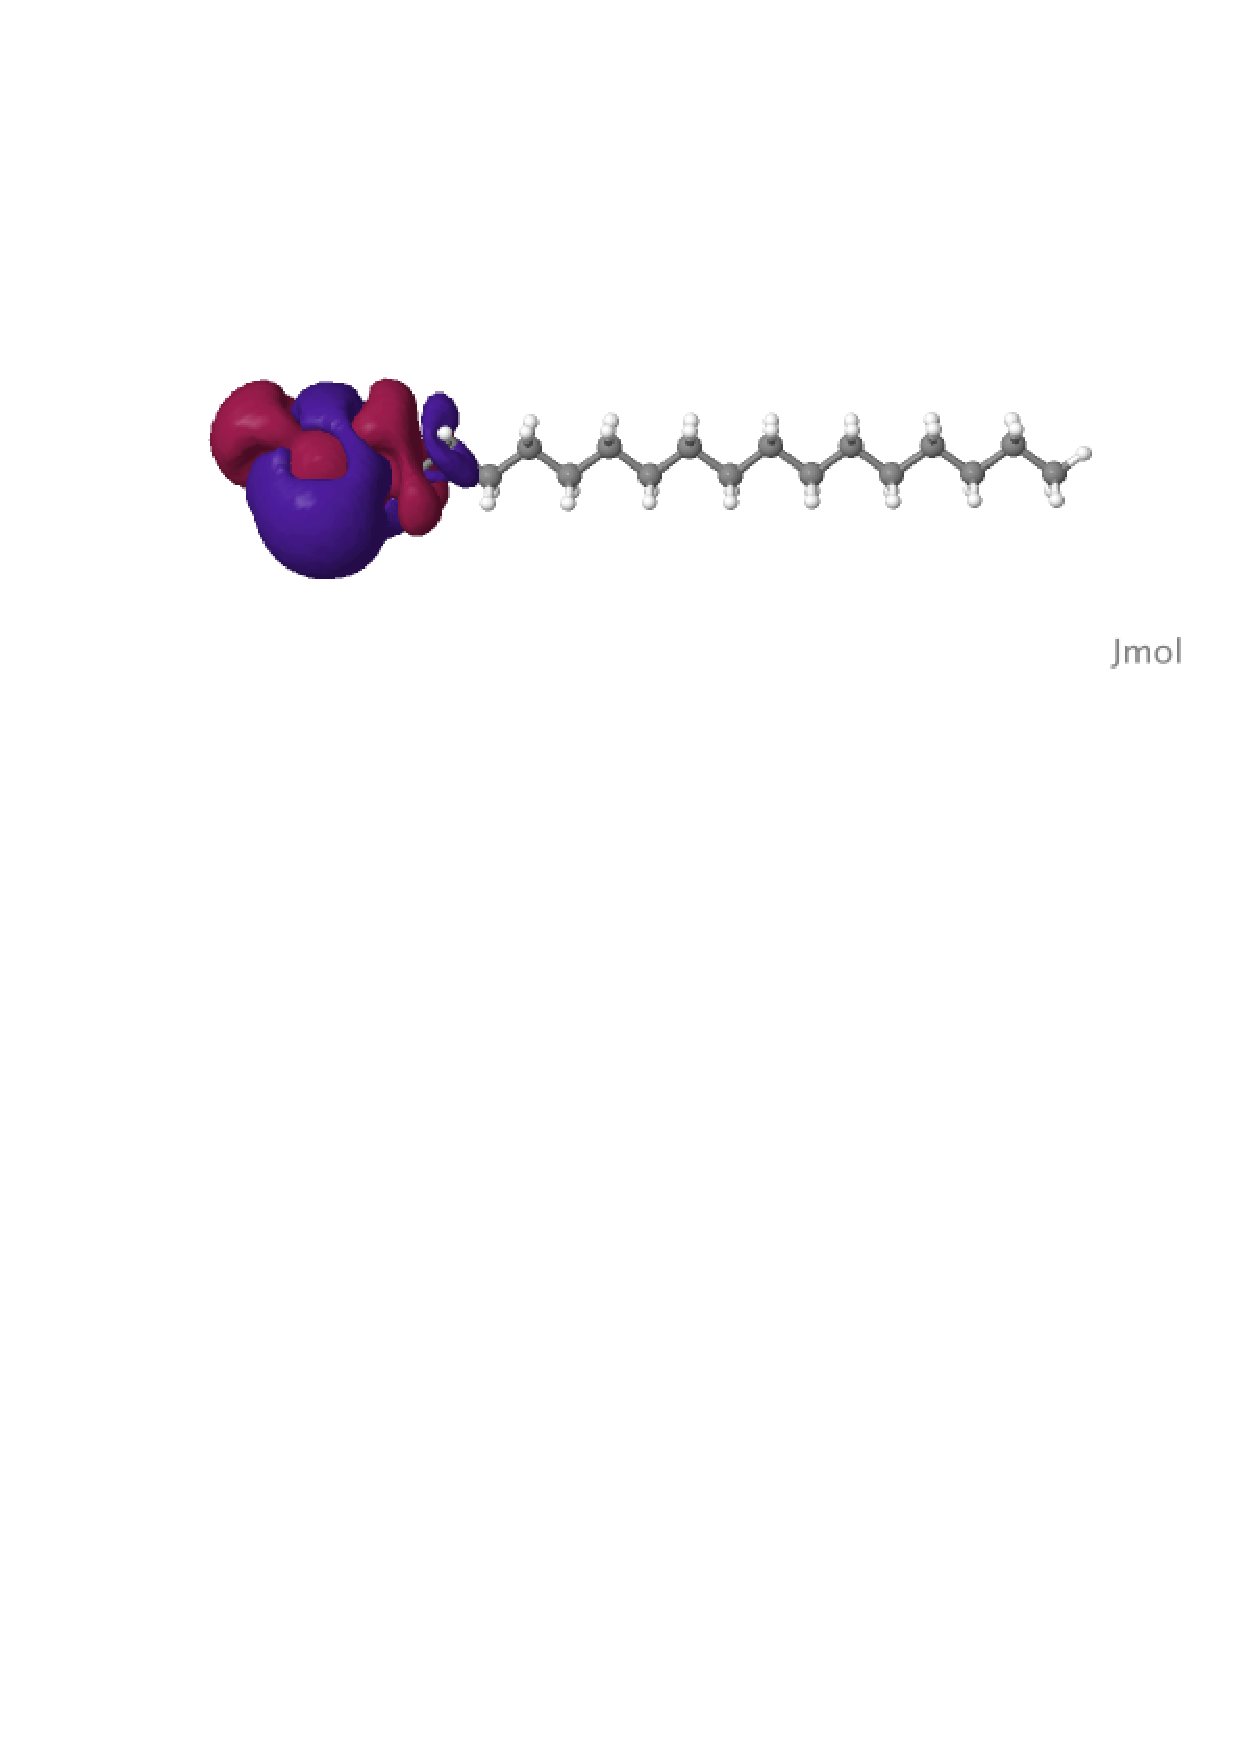
\includegraphics[scale=0.25, clip, viewport = 80 560 600 700]{figures/loc_orb_1.pdf}\\
    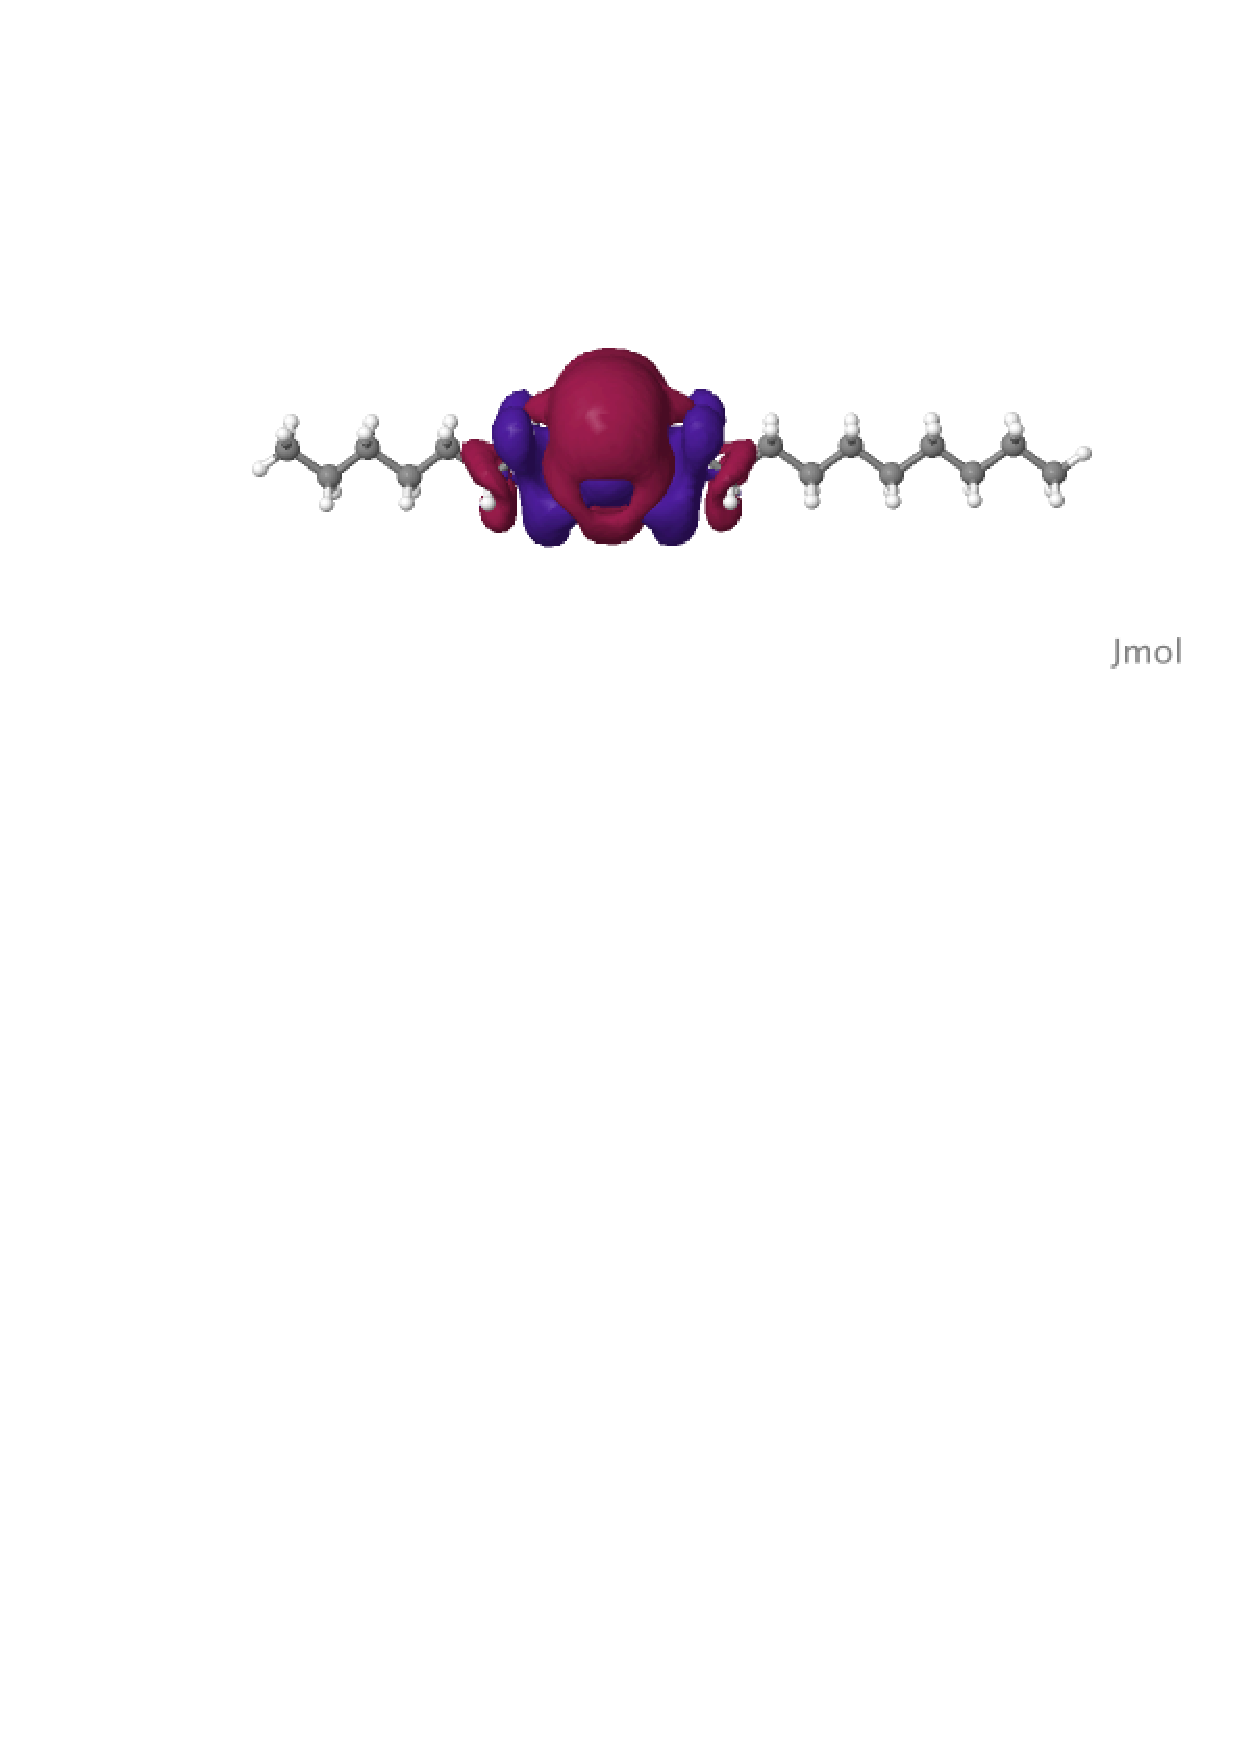
\includegraphics[scale=0.25, clip, viewport = 80 560 600 700]{figures/loc_orb_2.pdf}\\
    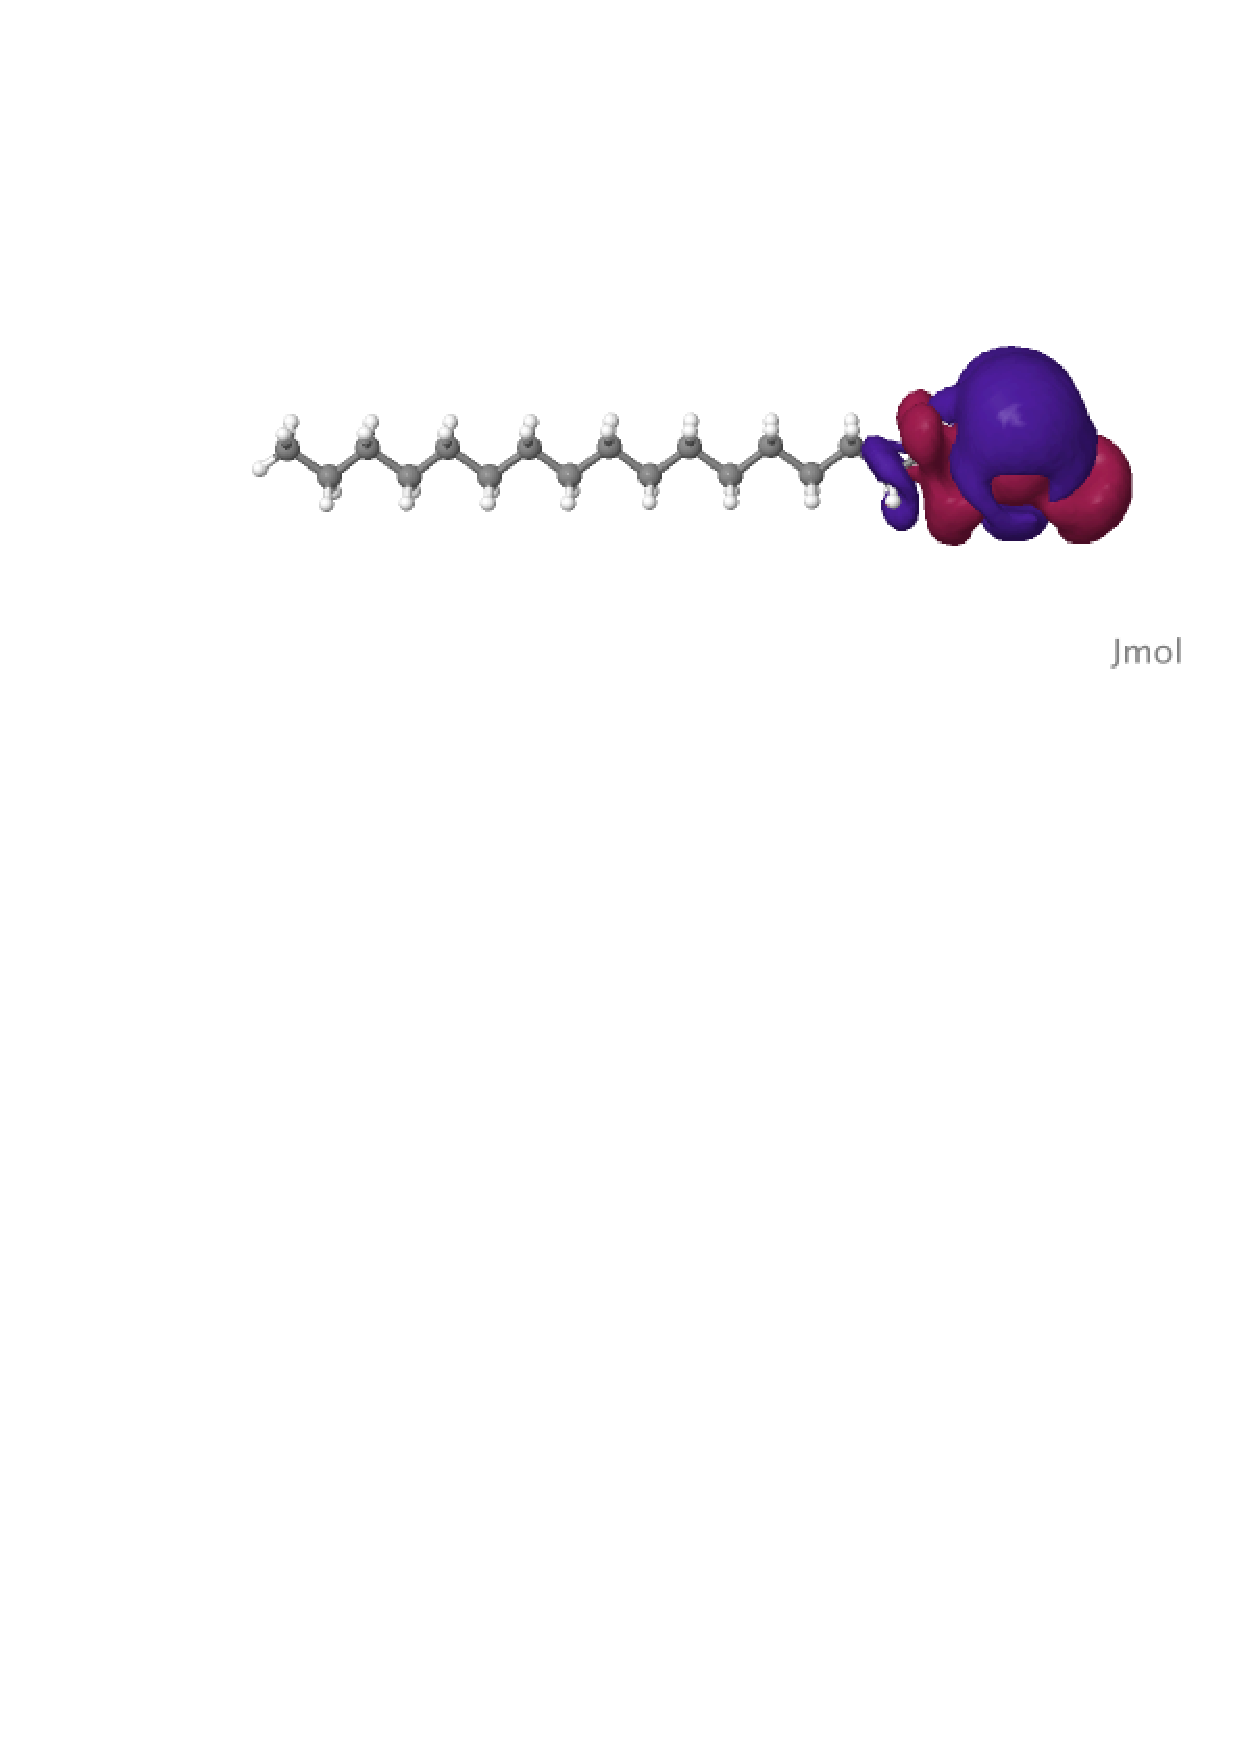
\includegraphics[scale=0.25, clip, viewport = 80 560 600 700]{figures/loc_orb_3.pdf}\\

    \vspace{2mm}

    \begin{equation}
        \nonumber
        \orbital_i =\ -2\Helm_i\Bigg[\potential \orbital_i
        - \sum_{j \neq i}\fockMat_{ij} \orbital_j\Bigg]
    \end{equation}
}
    \end{column}
    \end{columns}

    \vspace{4mm}

    \centering
    \tiny
    S.F. Boys,
    {\it Rev. Mod. Phys.},
    \textbf{32:296}
    (1960)\\
    J.M. Foster, S.F. Boys,
    {\it Rev. Mod. Phys.},
    \textbf{32:300}
    (1960)
\end{frame}

